\section{Linear parameter varying control}
\begin{frame}{Linear parameter varying control}{Classical approach}
\begin{columns}[T]
    \begin{column}{0.48\textwidth}
        \textbf{Nonlinear PMSM dynamics:}
            \begin{align*}
        L_d \frac{di_d}{dt} &= v_d - Ri_d \textcolor{red}{+p L_q\omega i_q} \\
        L_q\frac{di_q}{dt} &= v_q -Ri_q \textcolor{red}{-pL_d\omega i_d} -p \phi_f\omega
            \end{align*}

            \pause
            \vspace{0.2cm}
            \textbf{Feedback linearization:}
            \begin{equation*}
                \begin{cases}
                    v_d = u_d -pL_q\omega i_q\\
                    v_q = u_q +pL_d\omega i_d
                \end{cases}
            \end{equation*}
            \pause
    \end{column}
    \begin{column}{0.48\textwidth}
        \textbf{Linearized system:}
            \begin{equation*}
              \dot{x}= A x +B_u u
            \end{equation*}

            \pause
            \vspace{0.2cm}
            \textbf{Augmented state:}
            \begin{align*}
                \varepsilon_{i_d} &= \int_{0}^t (i_d^\# - i_d) d\tau\\
                \varepsilon_{i_q} &= \int_{0}^t (i_q^\# - i_q) d\tau
            \end{align*}

        \pause
        \vspace{0.2cm}
            \textbf{PI control law:}
            \begin{equation*}
                u = K x
            \end{equation*}
    \end{column}
\end{columns}
\end{frame}

\begin{frame}{Linear parameter varying control}{Proposed LPV approach}
\begin{columns}[T]
    \begin{column}{0.48\textwidth}
        \textbf{Nonlinear PMSM dynamics:}
            \begin{align*}
        L_d \frac{di_d}{dt} &= v_d - Ri_d \textcolor{red}{+p L_q\omega i_q} \\
        L_q \frac{di_q}{dt} &= v_q -Ri_q \textcolor{red}{-pL_d\omega i_d} -p \phi_f\omega
            \end{align*}

            \vspace{0.3cm}
            \textbf{Classical approach:}
            \begin{equation*}
                \xcancel{\begin{cases}
                    v_d = u_d -pL_q\omega i_q\\
                    v_q = u_q +pL_d\omega i_d
                \end{cases}}
            \end{equation*}
            \pause
    \end{column}
    \begin{column}{0.48\textwidth}
        \textbf{LPV model:}
            \begin{align*}
               \dot{x} &= A(\omega)x +B_u u\\
               \omega &\in \left[ \omega_{\min},\, \omega_{\max} \right]
            \end{align*}

            \pause
            \vspace{0.2cm}
            \textbf{Augmented state:}
            \begin{equation*}
                x = \begin{bmatrix}
                i_d & i_q & \varepsilon_{i_d}& \varepsilon_{i_q}
            \end{bmatrix}^\top
            \end{equation*}

            \pause
            \vspace{0.2cm}
            \textbf{Parameter dependant control:}
            \begin{equation*}
                v_{dq} =  K (\omega)x
            \end{equation*}
    \end{column}
\end{columns}
\end{frame}

\begin{frame}{Linear parameter varying control}{LPV specification: constrained-$\mathcal{H}_2$}
    \textbf{Control synthesis problem:} Design a parameter-dependent controller $K(\omega)$ that ensures closed-loop stability and performance for all speed trajectories $\omega(t)$.

    \vspace{0.4cm}
    %\begin{columns}[c]
    %\begin{column}{0.5\textwidth}
        %%%%%%%%% LMI regions figure
    \begin{figure}[]
        \centering
        \begin{tikzpicture}[scale=2.2]
    \def\xmin{-1.4cm} \def\xmax{0.5cm}
    \def\ymin{-1.4cm} \def\ymax{1cm}

    \draw [thick,->] (\xmin,0) -- (\xmax,0) node [anchor = west]{$\operatorname{Re}(z)$};
    \draw [thick,->] (0,\ymin) -- (0,\ymax) node [anchor = south]{$\operatorname{Im}(z)$};
    \begin{scope}
      \clip (-1cm,-1cm) rectangle (-0.3cm,1cm);
      \fill[gray!30,opacity=0.6] (-0.3cm,0.3cm) -- (-0.3cm,-0.3cm) -- (-1cm,-1cm) -- (-1cm,1cm) -- cycle;
    \end{scope}
    \draw [darkGreen,line width= 0.5mm] (-0.3cm,-0.3cm) -- (-0.3cm,0.3cm);
    \draw [darkGreen,line width= 0.5mm,dashed] (-0.3cm,0.3cm) -- (-0.3cm,1cm);
    \draw [darkGreen,line width= 0.5mm,dashed] (-0.3cm,-0.3cm) -- (-0.3cm,-1cm);
    \draw [darkBlue,line width= 0.5mm, dashed] (0cm,0cm) -- (-0.3cm,0.3cm);
    \draw [darkBlue,line width= 0.5mm] (-0.3cm,0.3cm) -- (-1cm,1cm);
    \draw [darkBlue,line width= 0.5mm, dashed] (-1cm,1cm) -- (-1cm,1cm) node [pos=1,above left] {$\beta$};
    \draw [darkBlue,line width= 0.5mm, dashed] (0cm,0cm) -- (-0.3cm,-0.3cm);
    \draw [darkBlue,line width= 0.5mm] (-0.3cm,-0.3cm) -- (-1cm,-1cm);
    \draw[->,darkBlue,line width=0.4mm] (-0.15,0.15) arc[start angle=145, end angle=175, radius=0.25cm];
    \node[text=darkBlue] at (-0.3,0.2) {$\psi$};
    \draw[<->,darkGreen,line width=0.4mm] (-0.05,-0.9cm) -- (-0.25cm,-0.9cm) node[midway, below, text=darkGreen] {$\alpha$};
    % Arrow pointing to the gray region from the left
    \draw [->,red,line width=0.4mm] (-1.3cm,0.5cm) -- (-0.6cm,0cm);
    \node[text=red,align=center] at (-1.6cm,0.8cm) {\tiny Minimize\\[-0.05cm]\tiny performance\\[-0.05cm]\tiny criterion};
        \end{tikzpicture}
    \end{figure}
    %\end{column}

    % \begin{column}{0.45\textwidth}
    % \textbf{Design specifications:}

    % \vspace{0.3cm}
    % \textbf{Hard constraints:}

    % Pole placement in $\mathbb{D}_\alpha \cap \mathbb{D}_\beta$
    % \begin{itemize}
    %     \item \textcolor{darkGreen}{$\mathbb{D}_\alpha$:} minimum decay rate
    %     \item \textcolor{darkBlue}{$\mathbb{D}_\beta$:} damping ratio
    % \end{itemize}

    % \vspace{0.4cm}
    % \textbf{Soft constraint:}

    % Minimize $\|H_{wz}\|_{\mathcal{H}_2}^2$ performance
    % \end{column}
    % \end{columns}

     \vspace{0.4cm}
    \begin{center}
    \textbf{This is formulated as a convex optimization problem involving LMIs.}
    \end{center}
\end{frame}

\begin{frame}{Linear parameter varying control}{Proposed implementation: Constrained $\mathcal{H}_2$ LPV control}
    \textbf{Proposed approach:} LPV controller with "frozen" pole placement and $\mathcal{H}_2$ performance optimization.

       \begin{figure}
\begin{psfrags}
\def\textsize{.7}

\psfrag{Vr}[c][c][\textsize]{\color{blue4}$\rho^\#$}
\psfrag{thm}[c][c][\textsize]{\color{blue4}$\theta$}
\psfrag{wm}[c][c][\textsize]{\color{green4}$\omega$}
\psfrag{iabc}[c][c][\textsize]{\color{blue4}$i_{abc}$}
\psfrag{idq}[c][c][\textsize]{\color{blue4}$i_{dq}$}
\psfrag{vabcr}[c][c][\textsize]{\color{blue4}$v_{abc}^\#$}
\psfrag{vdq2}[c][c][\textsize]{\color{blue4}$v_{dq}^\#$}
\psfrag{dq}[c][c][.5]{\color{blue4}${dq}$}
\psfrag{abc}[c][c][.5]{\color{blue4}${abc}\quad$}
\psfrag{S}[c][c][\textsize]{\color{green4}$S_{abc}$}
\psfrag{ParkInv}[c][c][.5]{}
\psfrag{Park}[c][c][.5]{}
\psfrag{ref}[c][c][\textsize]{\color{cyan4}$\omega^\#$}

\psfrag{MLI}[c][c][.4]{\color{blue4}Modulation}
\psfrag{Onduleur}[c][c][\textsize]{\color{red4}Inverter}
\psfrag{PMSM}[c][c][\textsize]{\color{red4}PMSM}

\psfrag{V}[c][c][\textsize]{\color{red4}$v_{abc}$}
\psfrag{th}[c][c][\textsize]{\color{red4}$\theta$}
\psfrag{w}[c][c][\textsize]{\color{red4}$\omega$}
\newcommand{\sat}{\mathrm{sat}}

\psfrag{Dynamique}[c][c][\textsize]{\color{green4}Dynamic}
\psfrag{Asservissement}[c][c][\textsize]{\color{blue4}control}
\psfrag{Elec}[c][c][\textsize]{\color{blue4}Electrical}
\psfrag{Dynamique2}[c][c][\textsize]{\color{blue4}Dynamic}
\psfrag{Asservissement2}[c][c][\textsize]{\color{green4}control}
\psfrag{Meca}[c][c][\textsize]{\color{green4}Mechanical}
\psfrag{CapW}[c][c][\textsize]{\color{green2}Mechanical}

\psfrag{Idqr2}[c][c][\textsize]{\color{green4}{$i_{dq}^\#$}}
\psfrag{Idqr}[c][c][\textsize]{\color{green4}${i_{dq}^\#}$}
\psfrag{vdqr}[c][c][\textsize]{\color{blue4}$\sat({v_{dq}^\#})$}
\psfrag{+r}[c][c][\textsize]{\color{red4}$+$}
\psfrag{-r}[c][c][\textsize]{\color{red4}$-$}
\psfrag{+v}[c][c][\textsize]{\color{blue4}$+$}
\psfrag{-v}[c][c][\textsize]{\color{blue4}$-$}
\psfrag{+b}[c][c][\textsize]{\color{green4}$+$}
\psfrag{-b}[c][c][\textsize]{\color{green4}$-$}
\psfrag{ref1}[c][c][\textsize]{\color{blue4}$\frac{1}{s}$}
\psfrag{ref2}[c][c][\textsize]{\color{blue4}$K_i$}
\psfrag{ref3}[c][c][\textsize]{\color{blue4}$K_p$}
\psfrag{eq}[c][c][\textsize]{\color{blue4}$K_{dq}$}
\psfrag{x}[c][c][\textsize]{\color{blue4}$\times$}
\psfrag{vrep}[c][c][\textsize]{\color{blue4}$\varepsilon_{dq}$}
\psfrag{vdq}[c][c][\textsize]{\color{blue4}$v_{dq}$}

\psfrag{TSM}[l][c][.7]{\color{green4}$F_{s,m}= 1$kHz}
\psfrag{TSE}[l][c][.7]{\color{blue4}$F_{s,e}= 20$kHz}

\psfrag{Embedded}[l][c][1]{\color{red}Embedded code}

\includegraphics[width = \textwidth]{pictures/ControlFOCLPV.eps}
\end{psfrags}
\end{figure}
\end{frame}


\begin{frame}{Linear parameter varying control}{Classical implementation: PI + Feedback linearization}
    \textbf{Classical approach:} PI controller with feedback linearization to cancel nonlinearities.

       \begin{figure}
\begin{psfrags}
\def\textsize{.7}

\psfrag{Vr}[c][c][\textsize]{\color{blue4}$\rho^\#$}
\psfrag{thm}[c][c][\textsize]{\color{blue4}$\theta$}
\psfrag{wm}[c][c][\textsize]{\color{green4}$\omega$}
\psfrag{iabc}[c][c][\textsize]{\color{blue4}$i_{abc}$}
\psfrag{idq}[c][c][\textsize]{\color{blue4}$i_{dq}$}
\psfrag{vabcr}[c][c][\textsize]{\color{blue4}$v_{abc}^\#$}
\psfrag{vdq2}[c][c][\textsize]{\color{blue4}$v_{dq}^\#$}
\psfrag{dq}[c][c][.5]{\color{blue4}${dq}$}
\psfrag{abc}[c][c][.5]{\color{blue4}${abc}\quad$}
\psfrag{S}[c][c][\textsize]{\color{green4}$S_{abc}$}
\psfrag{ParkInv}[c][c][.5]{}
\psfrag{Park}[c][c][.5]{}
\psfrag{ref}[c][c][\textsize]{\color{cyan4}$\omega^\#$}

\psfrag{MLI}[c][c][.4]{\color{blue4}Modulation}
\psfrag{Onduleur}[c][c][\textsize]{\color{red4}Inverter}
\psfrag{PMSM}[c][c][\textsize]{\color{red4}PMSM}

\psfrag{V}[c][c][\textsize]{\color{red4}$v_{abc}$}
\psfrag{th}[c][c][\textsize]{\color{red4}$\theta$}
\psfrag{w}[c][c][\textsize]{\color{red4}$\omega$}
\newcommand{\sat}{\mathrm{sat}}

\psfrag{Dynamique}[c][c][\textsize]{\color{green4}Dynamic}
\psfrag{Asservissement}[c][c][\textsize]{\color{blue4}control}
\psfrag{Elec}[c][c][\textsize]{\color{blue4}Electrical}
\psfrag{Dynamique2}[c][c][\textsize]{\color{blue4}Dynamic}
\psfrag{Asservissement2}[c][c][\textsize]{\color{green4}control}
\psfrag{Meca}[c][c][\textsize]{\color{green4}Mechanical}
\psfrag{CapW}[c][c][\textsize]{\color{green2}Mechanical}

\psfrag{Idqr2}[c][c][\textsize]{\color{green4}{$i_{dq}^\#$}}
\psfrag{Idqr}[c][c][\textsize]{\color{green4}${i_{dq}^\#}$}
\psfrag{vdqr}[c][c][\textsize]{\color{blue4}$\sat({v_{dq}^\#})$}
\psfrag{+r}[c][c][\textsize]{\color{red4}$+$}
\psfrag{-r}[c][c][\textsize]{\color{red4}$-$}
\psfrag{+v}[c][c][\textsize]{\color{blue4}$+$}
\psfrag{-v}[c][c][\textsize]{\color{blue4}$-$}
\psfrag{+b}[c][c][\textsize]{\color{green4}$+$}
\psfrag{-b}[c][c][\textsize]{\color{green4}$-$}
\psfrag{ref1}[c][c][\textsize]{\color{blue4}$\frac{1}{s}$}
\psfrag{ref2}[c][c][\textsize]{\color{blue4}$K_i$}
\psfrag{ref3}[c][c][\textsize]{\color{blue4}$K_p$}
\psfrag{eq}[c][c][\textsize]{\color{blue4}$pL_{dq}\mathcal{J}$}
\psfrag{x}[c][c][\textsize]{\color{blue4}$\times$}
\psfrag{vrep}[c][c][\textsize]{\color{blue4}$\varepsilon_{dq}$}
\psfrag{vdq}[c][c][\textsize]{\color{blue4}$v_{dq}$}

\psfrag{TSM}[l][c][.7]{\color{green4}$F_{s,m}= 1$kHz}
\psfrag{TSE}[l][c][.7]{\color{blue4}$F_{s,e}= 20$kHz}

\psfrag{Embedded}[l][c][1]{\color{red}Embedded code}

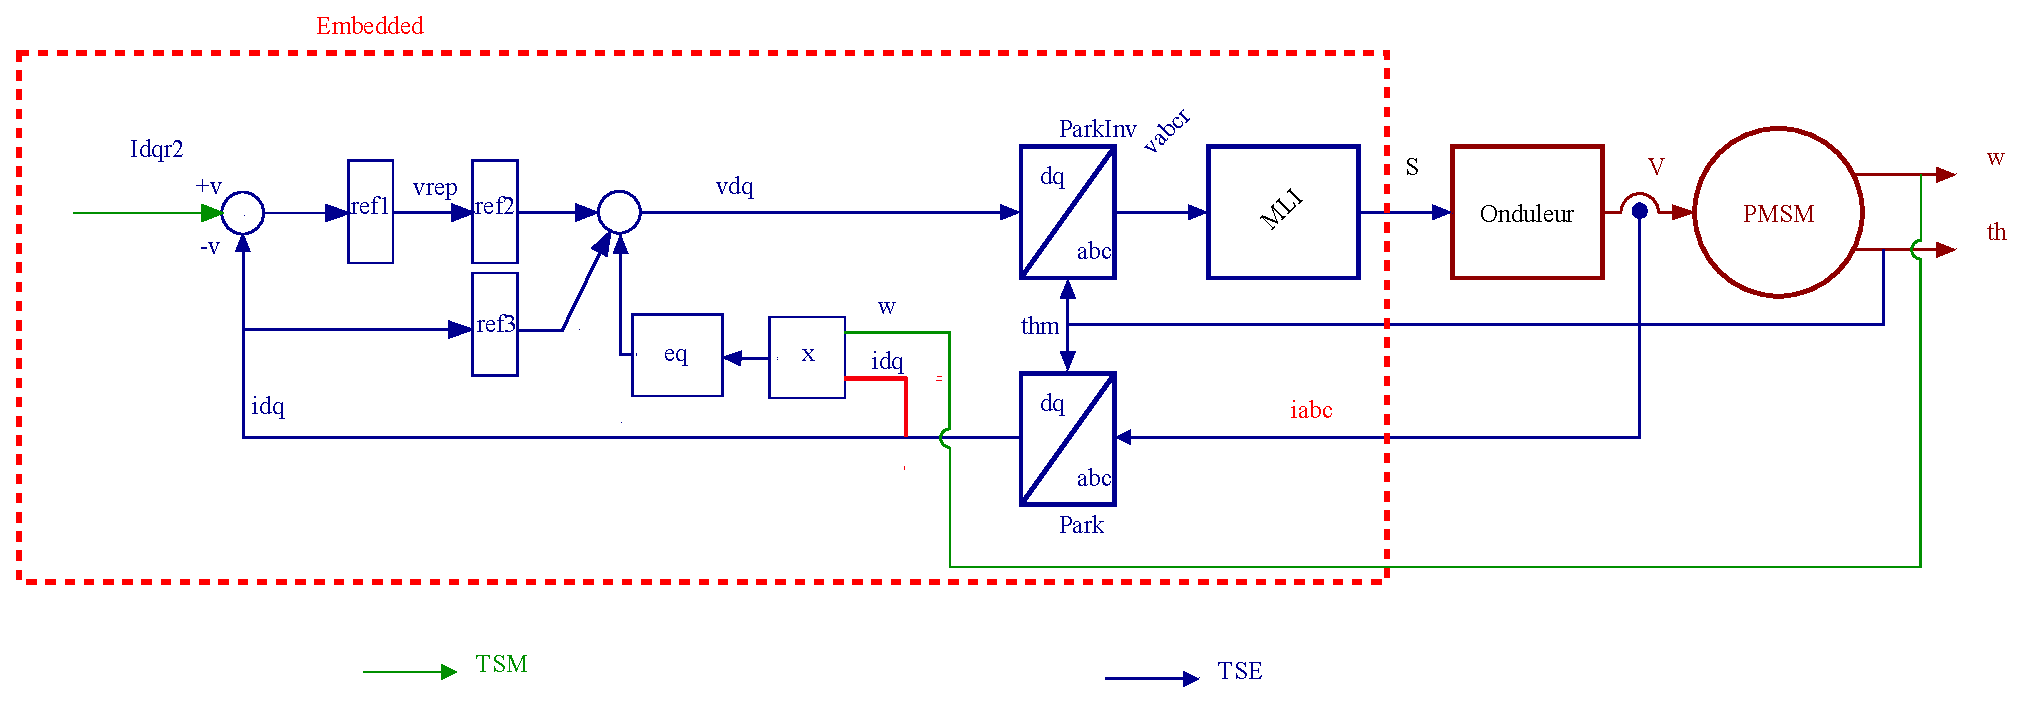
\includegraphics[width = \textwidth]{pictures/ControlFOCLPV_PI.eps}
\end{psfrags}
\end{figure}
\end{frame}


\begin{frame}{Linear parameter varying control}{Linearization-free approach}
    \textbf{Proposed approach:} Linearization-free control for PMSM through LMI-based synthesis.

    \vspace{0.3cm}
    \begin{columns}
        \begin{column}{0.5\textwidth}
        \textbf{PI + Feedback linearization}
           \begin{equation*}
               \begin{cases}
                    v_d = u_d -pL_q\omega i_q\\
                    v_q = u_q +pL_d\omega i_d
                \end{cases}
            \end{equation*}
            \vspace{0.2cm}
       \begin{itemize}
            \item[$-$] Direct current injection
            \item[$-$] High sensitivity to noise
            \item[$-$] No formal guarantees
        \end{itemize}
        \end{column}
        \begin{column}{0.5\textwidth}
            \textbf{Constrained-$\mathcal{H}_2$ LPV}
            \begin{equation*}
               \begin{cases}
                    v_d = u_d -K_d\omega \varepsilon_{i_q}\\
                    v_q = u_q +K_q\omega \varepsilon_{i_d}
                \end{cases}
            \end{equation*}
                    \vspace{0.2cm}
        \begin{itemize}
            \item[$+$] Reduced noise sensitivity
            \item[$+$] Stability via Lyapunov function
            \item[$+$] Performance guarantees
        \end{itemize}

        \end{column}
    \end{columns}
    \vspace{0.4cm}
    \begin{center}
    \begin{tikzpicture}
        \node[draw, rectangle, fill=green!10, minimum width=8cm, minimum height=0.8cm] {
            \begin{minipage}{7.5cm}
                \centering
                \small
                \textbf{Key difference:} $\omega i_{dq}$ (noisy) $\rightarrow$ $\omega \varepsilon_{i_{dq}}$ (filtered)
            \end{minipage}
        };
    \end{tikzpicture}
    \end{center}

\end{frame}


% \begin{frame}{LPV control}{Motivation}
%     \begin{figure}[H]
%     \centering
%     \includegraphics[trim=10cm 0.5cm 1cm 0.8cm, clip, width=0.85\textwidth]{pictures/LPV/control_law_corrected.eps}
%     \caption{Experiment validation for $\alpha = 49.98$}
%     \label{fig:alpha50}
%     \end{figure}
% \end{frame}

% \begin{frame}{LPV control: Motivation}
%     \textbf{Challenge with classical PI + feedback linearization:}

%     \vspace{0.3cm}
%     Classical approach is field-oriented control:
%      \begin{equation*}
%         v_{dq} = u_{dq} + pL_{dq}\omega \mathcal{J}i_{dq}
%     \end{equation*}

%     \vspace{0.2cm}
%     \begin{itemize}
%         \item[$-$] Injects current measurements directly into voltages
%         \item[$-$] Amplifies measurement noise, especially at high speeds
%         \item[$-$] No formal stability guarantee for time-varying speeds
%     \end{itemize}

%     \vspace{0.4cm}
%     \textbf{Goal:} Design a control that
%     \begin{itemize}
%         \item[$\checkmark$] Reduces noise sensitivity
%         \item[$\checkmark$] Guarantees performance for time-varying $\omega$
%         \item[$\checkmark$] Maintains intuitive tuning
%     \end{itemize}
% \end{frame}

% \begin{frame}{LPV systems framework}
%     \textbf{LPV state-space representation:}
%     \begin{align*}
%         \dot{x}(t) &= A(\rho(t))x(t) + B(\rho(t))u(t)\\
%         y(t) &= C(\rho(t))x(t) + D(\rho(t))u(t)
%     \end{align*}

%     where $\rho(t) \in \mathcal{R}^p$ is the scheduling parameter (measurable in real-time)

%     \vspace{0.3cm}
%     \textbf{Parameter-dependent controller:}
%     \begin{equation*}
%         u(t) = K(\rho(t))x(t)
%     \end{equation*}

%     \vspace{0.3cm}
%     \textbf{Key idea:} Use polytopic formulation
%     \begin{itemize}
%         \item Express system matrices as convex combinations at vertices
%         \item Check LMIs only at vertices (computationally tractable)
%         \item Use single quadratic Lyapunov function: $V(x) = x^\top P x$
%     \end{itemize}
% \end{frame}

% \begin{frame}{LPV model for IPMSM}
%     \textbf{Electrical dynamics with integral action:}
%     \begin{align*}
%         \dot{x} &= A(\omega)x + Bu + B_w w\\
%         z &= C_z x + D_z u
%     \end{align*}

%     where $x = [i_d,\, i_q,\, \varepsilon_{i_d},\, \varepsilon_{i_q}]^\top$

%     \vspace{0.3cm}
%     \textbf{Parameter-dependent matrix:}
%     \begin{equation*}
%         A(\omega) = A_c + A_l \omega
%     \end{equation*}

%     \vspace{0.2cm}
%     \textbf{Scheduling parameter:} $\omega \in \mathbf{\Omega} = [\omega_{min}, \omega_{max}]$

%     \vspace{0.3cm}
%     \textbf{Controller structure:}
%     \begin{equation*}
%         u = K(\omega)x = K_{pi}x + K_f \omega x
%     \end{equation*}
% \end{frame}

% \begin{frame}{Polytopic LPV formulation}
%     \textbf{Two vertices for speed range:} $\theta_1 = \omega_{min}$, $\theta_2 = \omega_{max}$

%     \vspace{0.3cm}
%     \textbf{Polytopic decomposition:}
%     \begin{equation*}
%         \omega = \sum_{i=1}^{2} \lambda_i \theta_i, \quad
%         A(\omega) = \sum_{i=1}^{2} \lambda_i A_i, \quad
%         K(\omega) = \sum_{i=1}^{2} \lambda_i K_i
%     \end{equation*}

%     with $\lambda_i \geq 0$ and $\lambda_1 + \lambda_2 = 1$

%     \vspace{0.3cm}
%     \textbf{Vertex gains:}
%     \begin{align*}
%         K_1 &= K_{pi} + K_f \omega_{min}\\
%         K_2 &= K_{pi} + K_f \omega_{max}
%     \end{align*}

%     \vspace{0.3cm}
%     $\Rightarrow$ \textbf{Finite LMI problem:} Check conditions only at $\omega_{min}$ and $\omega_{max}$
% \end{frame}

% \begin{frame}{Constrained-$\mathcal{H}_2$ LPV synthesis}
%     \textbf{Optimization problem at each vertex $i \in \{1,2\}$:}

%     \vspace{0.2cm}
%     \small
%     \begin{align*}
%         \min_{X,Y_i,W,\gamma} \quad & \gamma\\
%         \text{s.t.} \quad & \langle A_iX + BY_i \rangle_S + 2\alpha X \prec 0 \quad \text{(decay rate)}\\
%         & \begin{bmatrix}
%             \beta \langle A_iX + BY_i \rangle_S & (*)^\top\\
%             (A_iX + BY_i)^\top - (A_iX + BY_i) & \beta \langle A_iX + BY_i \rangle_S
%         \end{bmatrix} \prec 0\\
%         & \text{(damping)}\\
%         & \mathcal{H}_2 \text{ conditions} \quad \text{(noise minimization)}
%     \end{align*}

%     \normalsize
%     \vspace{0.2cm}
%     \textbf{Result:} Controller $K_i = Y_i X^{-1}$ guarantees:
%     \begin{itemize}
%         \item Performance in $\mathcal{D}_\alpha \cap \mathcal{D}_\beta$ for all $\omega \in \mathbf{\Omega}$
%         \item Minimized noise sensitivity
%     \end{itemize}
% \end{frame}

% \begin{frame}{Control structures comparison}
%     \begin{columns}[t]
%     \begin{column}{0.5\textwidth}
%         \textbf{PI + feedback linearization:}
%         \begin{equation*}
%             v_{dq} = u_{dq} + pL_{dq}\omega \mathcal{J}i_{dq}
%         \end{equation*}

%         \vspace{0.2cm}
%         \begin{itemize}
%             \item[$-$] Direct current injection
%             \item[$-$] High noise at high $\omega$
%             \item[$+$] Simple to implement
%         \end{itemize}
%     \end{column}

%     \begin{column}{0.5\textwidth}
%         \textbf{Constrained-$\mathcal{H}_2$ LPV:}
%         \begin{equation*}
%             v_{dq} = u_{dq} + K_{dq}\mathcal{J}\omega \varepsilon_{i_{dq}}
%         \end{equation*}

%         \vspace{0.2cm}
%         \begin{itemize}
%             \item[$+$] Uses integral (low-pass filter)
%             \item[$+$] Reduced noise sensitivity
%             \item[$+$] Formal stability guarantee
%         \end{itemize}
%     \end{column}
%     \end{columns}

%     \vspace{0.4cm}
%     \begin{center}
%     \begin{tikzpicture}
%         \node[draw, rectangle, fill=green!10, minimum width=8cm, minimum height=0.8cm] {
%             \begin{minipage}{7.5cm}
%                 \centering
%                 \small
%                 \textbf{Key difference:} $\omega i_{dq}$ (noisy) $\rightarrow$ $\omega \varepsilon_{i_{dq}}$ (filtered)
%             \end{minipage}
%         };
%     \end{tikzpicture}
%     \end{center}
% \end{frame}
% \begin{frame}{Linear parameter varying control}{Frozen parameter pole analysis}
%         \textbf{How do poles move with varying speed?}
%     \begin{columns}[]
%     \begin{column}{0.5\textwidth}
%     \textbf{PI control}
%         \only<1>{\includegraphics[width=0.9\columnwidth]{LPV_vs_PI/PI_0.eps}}
%         \only<2>{\includegraphics[width=0.9\columnwidth]{LPV_vs_PI/PI_200.eps}}
%         \only<3>{\includegraphics[width=0.9\columnwidth]{LPV_vs_PI/PI_400.eps}}
%         \only<4>{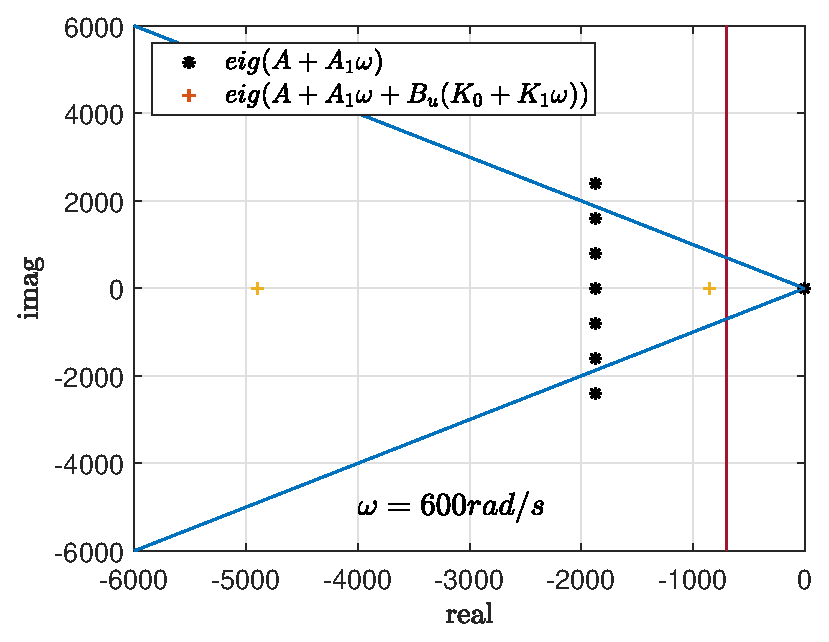
\includegraphics[width=0.9\columnwidth]{LPV_vs_PI/PI_600.eps}}
%         \only<5>{\includegraphics[width=0.9\columnwidth]{LPV_vs_PI/PI_800.eps}}
%     \small{\begin{equation*}
%                 \begin{cases}
%                 v_d = [K_{11}i_d +K_{13}\varepsilon_{i_{d}}]-\textcolor{red}{pL}\omega i_q\\
%                 v_q = [K_{22}i_q +K_{44}\varepsilon_{i_{q}}]+\textcolor{red}{pL} \omega i_d
%                 \end{cases}
%             \end{equation*}
%         }
%     \end{column}
%     \begin{column}{0.5\textwidth}

%     \textbf{Constrained LPV $\mathcal{H}_2$}

%         \only<1>{\includegraphics[width=0.9\columnwidth]{LPV_vs_PI/LPV_0.eps}}
%         \only<2>{\includegraphics[width=0.9\columnwidth]{LPV_vs_PI/LPV_200.eps}}
%         \only<3>{\includegraphics[width=0.9\columnwidth]{LPV_vs_PI/LPV_400.eps}}
%         \only<4>{\includegraphics[width=0.9\columnwidth]{LPV_vs_PI/LPV_600.eps}}
%         \only<5>{\includegraphics[width=0.9\columnwidth]{LPV_vs_PI/LPV_800.eps}}
%         \small{\begin{equation*}
%                 \begin{cases}
%                 v_d = [K_{11}i_d +K_{13}\varepsilon_{i_{d}}]-\textcolor{red}{K_d} \omega \colorbox{SpringGreen}{$\varepsilon_{i_{d}}$}\\
%                 v_q = [K_{22}i_q +K_{44} \varepsilon_{i_{q}}]+\textcolor{red}{K_q} \omega \colorbox{SpringGreen}{$\varepsilon_{i_{q}}$}
%                 \end{cases}
%         \end{equation*}
%        % $\:\varepsilon_{i_{d}=} \int_0^t (i_d - i_{d}^\#) dt $, $\varepsilon_{i_{q}=} \int_0^t (i_q - i_{q}^\#) dt $
%         }
%     \end{column}
%     \end{columns}
% \end{frame}

\begin{frame}{Linear parameter varying control}{Experimental validation}
\begin{columns}
    \begin{column}{0.5\textwidth}
        \begin{figure}[H]
        \centering
        \includegraphics[trim={0cm 5cm 2cm 0cm},clip,width=1\columnwidth]{pictures/Banc_IPMSM.eps}
        \caption{PMSM test bench.}
        \label{fig:bancIPMSM_sec3}
    \end{figure}    
    \end{column}
    \begin{column}{0.5\textwidth}
        \vspace{-1.5cm}
                     \begin{figure}
             \centering
         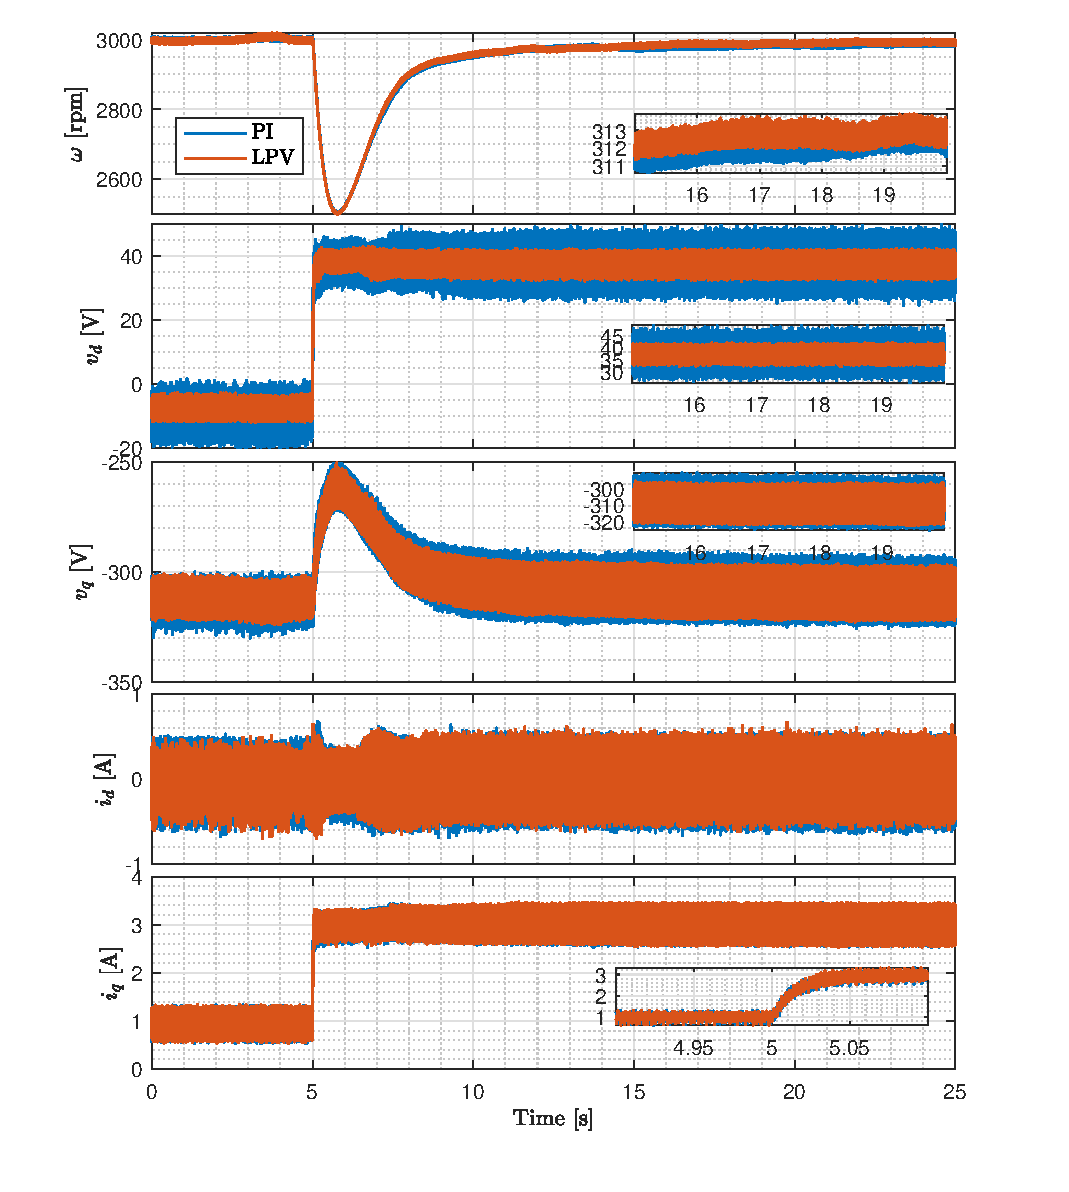
\includegraphics[trim={0.8cm 0.7cm 1.5cm 0.2cm},clip,width=1\columnwidth]{pictures/current_step.eps}
            \end{figure}
    \end{column}
\end{columns}
    

 %   \vspace{0.3cm}

   % \begin{columns}
     % \begin{column}{0.5\textwidth}

        % \end{column}
      %  \begin{column}{0.5\textwidth}
        % % %   \only<1>{  \begin{figure}
        % % %     \centering
        % % %     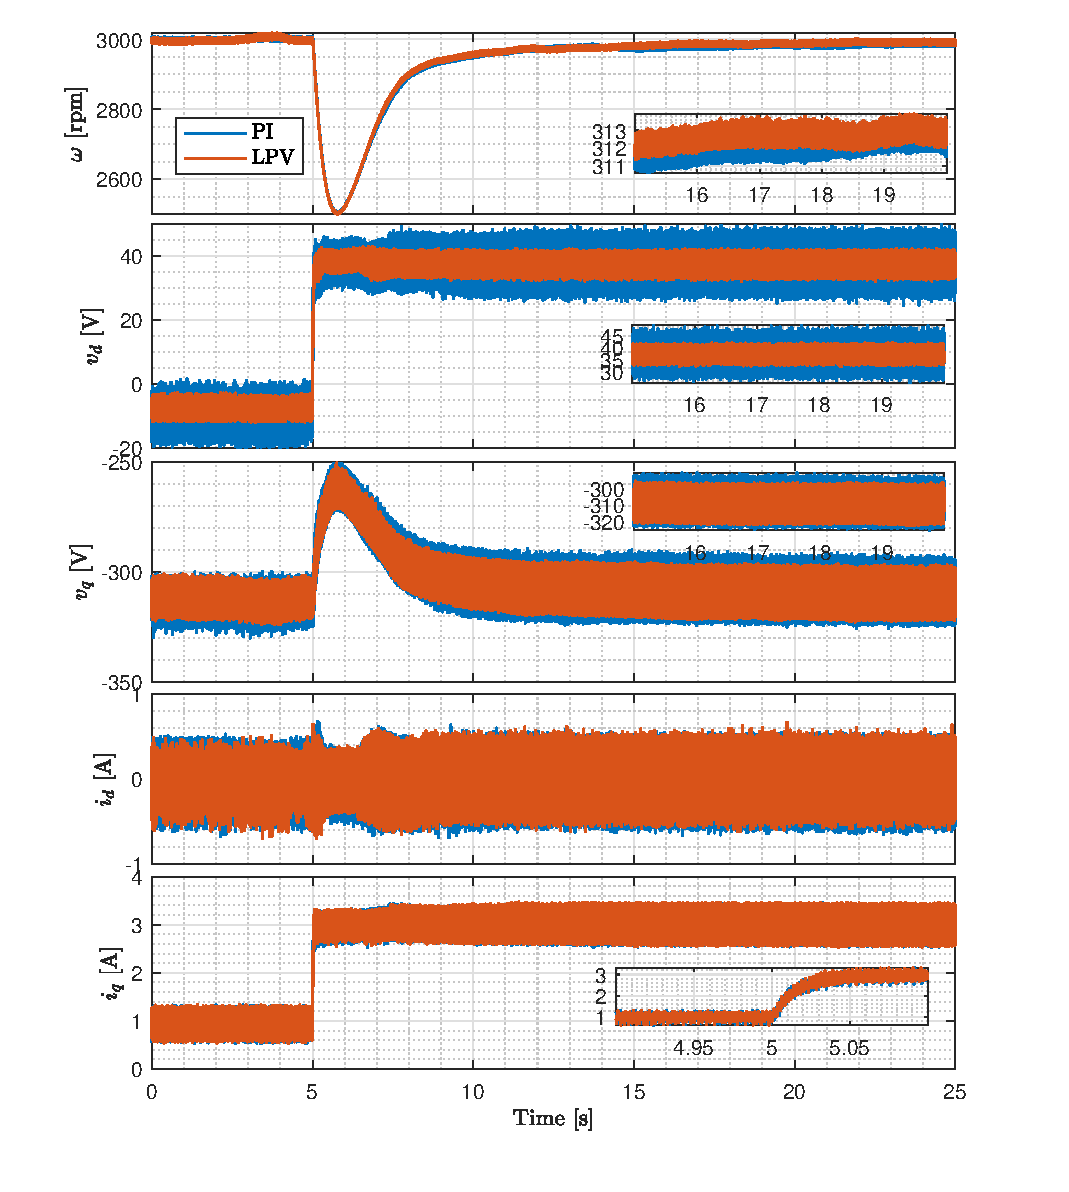
\includegraphics[trim={0.4cm 8.9cm 1.4cm 10.2cm},clip,width=0.7\textwidth]{pictures/current_step.eps}
        % % %     \end{figure} }
            
        % % %     \only<2>{  
        % % %     \begin{figure}
        % % %         \centering
        % % %         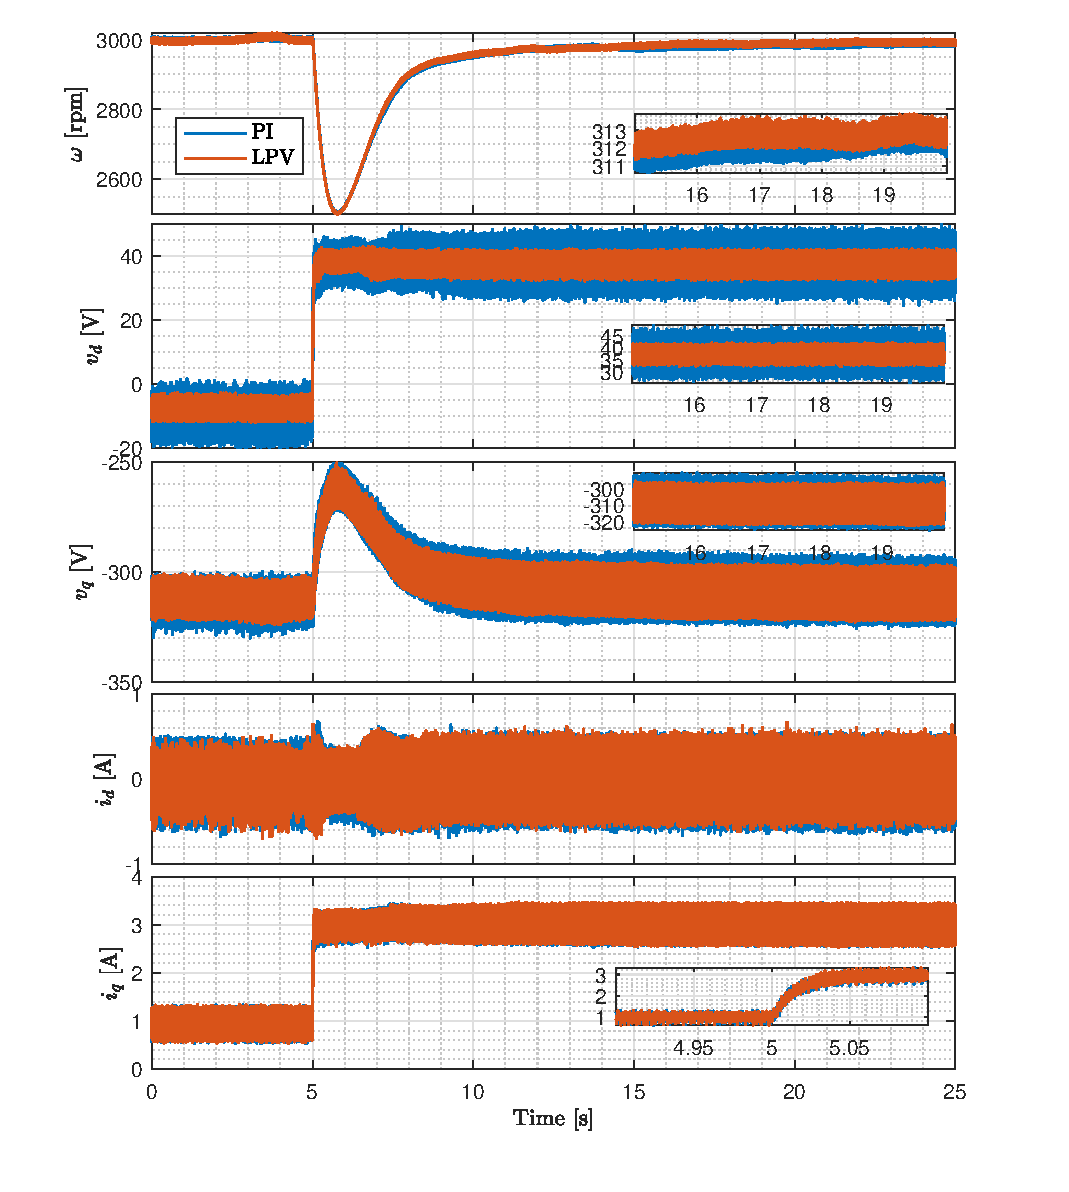
\includegraphics[trim={0.4cm 1.4cm 1.4cm 11.5cm},clip,width=0.7\textwidth]{pictures/current_step.eps}
        % % %     \end{figure}}
            %trim={<left> <bottom> <right> <top>}
       % \end{column}
  %  \end{columns}
\end{frame}

% \begin{frame}{Frozen parameter pole analysis}
%     \textbf{How do poles move with varying speed?}

%     \vspace{0.3cm}
%     \begin{columns}[t]
%     \begin{column}{0.5\textwidth}
%         \centering
%         \textbf{PI feedback linearization}

%         \vspace{0.2cm}
%         \begin{itemize}
%             \item Cancels speed-dependent terms
%             \item Fixed pole locations
%             \item Independent of $\omega$
%         \end{itemize}

%         \vspace{0.2cm}
%         \small
%         \textcolor{gray}{(See figure in thesis)}
%     \end{column}

%     \begin{column}{0.5\textwidth}
%         \centering
%         \textbf{Constrained-$\mathcal{H}_2$ LPV}

%         \vspace{0.2cm}
%         \begin{itemize}
%             \item Adapts to speed variation
%             \item Poles move within $\mathcal{D}_\alpha \cap \mathcal{D}_\beta$
%             \item Preserves natural dynamics
%         \end{itemize}

%         \vspace{0.2cm}
%         \small
%         \textcolor{gray}{(See figure in thesis)}
%     \end{column}
%     \end{columns}

%     \vspace{0.4cm}
%     \textbf{Note:} Analysis at "frozen" speeds gives intuition, but LPV guarantees performance for time-varying $\omega$
% \end{frame}

% \begin{frame}{Sensitivity function analysis}
%     \textbf{Transfer function from sensor noise $w_d$ to:}

%     \vspace{0.3cm}
%     \begin{itemize}
%         \item \textbf{Control input $v_q$:}
%         \begin{itemize}
%             \item Constrained-$\mathcal{H}_2$ shows better roll-off at high frequencies
%             \item Reduced noise amplification compared to PI
%         \end{itemize}

%         \vspace{0.2cm}
%         \item \textbf{Performance output $i_q$:}
%         \begin{itemize}
%             \item Better decoupling between d-q axes
%             \item Lower cross-axis sensitivity
%         \end{itemize}
%     \end{itemize}

%     \vspace{0.3cm}
%     \textbf{Why better high-frequency attenuation?}
%     \begin{itemize}
%         \item $\mathcal{H}_2$ optimization minimizes energy across spectrum
%         \item Integral action provides natural low-pass filtering
%     \end{itemize}

%     \vspace{0.2cm}
%     $\Rightarrow$ \textbf{More robust and noise-resilient control at no added computational cost}
% \end{frame}

% \begin{frame}{Experimental validation: Setup}
%     \textbf{Test bench:} IPMSM with dSpace MicroLabBox

%     \vspace{0.3cm}
%     \textbf{Two experiments:}

%     \vspace{0.2cm}
%     \textbf{1) Torque step at constant speed (3000 rpm):}
%     \begin{itemize}
%         \item Evaluate transient behavior
%         \item Both controls tuned for same dynamics
%     \end{itemize}

%     \vspace{0.3cm}
%     \textbf{2) Speed ramp (500 to 4000 rpm):}
%     \begin{itemize}
%         \item Evaluate steady-state at various speeds
%         \item Covers MTPA and field-weakening regions
%     \end{itemize}

%     \vspace{0.3cm}
%     \textbf{Measured signals:} $\omega$, $v_d$, $v_q$, $i_d$, $i_q$

%     \vspace{0.2cm}
%     \textbf{Comparison:} PI + feedback linearization vs. Constrained-$\mathcal{H}_2$ LPV
% \end{frame}

% \begin{frame}{Experimental results: Key findings}
%     \textbf{Voltage quality:}
%     \begin{itemize}
%         \item[$\checkmark$] \textbf{Smoother voltages $v_{dq}$} with constrained-$\mathcal{H}_2$
%         \item[$\checkmark$] Reduced high-frequency noise
%         \item[$\checkmark$] Especially visible on $v_d$ (higher $i_q$ amplitude)
%     \end{itemize}

%     \vspace{0.3cm}
%     \textbf{Current dynamics:}
%     \begin{itemize}
%         \item[$\checkmark$] \textbf{Identical $i_d$ and $i_q$ dynamics} for both methods
%         \item[$\checkmark$] Same transient response (as designed)
%         \item Both affected by same sensor noise (-20 dB for PI, -50 dB for $\mathcal{H}_2$)
%     \end{itemize}

%     \vspace{0.3cm}
%     \begin{center}
%     \begin{tikzpicture}
%         \node[draw, rectangle, fill=blue!10, minimum width=8cm, minimum height=0.8cm] {
%             \begin{minipage}{7.5cm}
%                 \centering
%                 \textbf{Same dynamics + Less noisy inputs = Better performance}
%             \end{minipage}
%         };
%     \end{tikzpicture}
%     \end{center}

%     \vspace{0.2cm}
%     \small
%     \textcolor{gray}{See detailed experimental plots in thesis: Figures 4.11 and 4.12}
% \end{frame}

\begin{frame}{Linear parameter varying control}{LPV control: Summary}
    \textbf{Contributions:}
    \begin{itemize}
        \item \textbf{Linearization-free control:} No exact cancellation needed
        \item \textbf{Performance guarantees:} Lyapunov certificate for time-varying $\omega$
        \item \textbf{Noise reduction:} filtering effect due to the  $\mathcal{H}_2$ optimization 
        \item \textbf{Experimental validation:} Confirmed on PMSM test bench
    \end{itemize}

    % \vspace{0.3cm}
    % \textbf{Advantages over classical PI:}
    % \begin{itemize}
    %     \item[$+$] Same computational cost (no additional online computation)
    %     \item[$+$] Maintains classical nested structure (easy integration)
    %     \item[$+$] Intuitive tuning via $\alpha$, $\beta$ parameters
    %     \item[$+$] Better noise rejection
    % \end{itemize}

    \vspace{0.3cm}
    \textbf{Other work:}
    \begin{itemize}
        \item Robustness to parametric uncertainty $\rightarrow$  norm-bounded parametric  uncertainty
    \end{itemize}
\end{frame}

% \begin{frame}{Polynomial transformation for voltage constraint}
%     The polynomial form for a given  IPMSM with parameters $R$ $L_d$, $L_q$, $\phi_f$, $p$:
%     \begin{equation*}
%         h(i_d, \tau, \omega) = a_4(\tau,\omega) i_d^4 + a_3(\tau,\omega) i_d^3 + a_2(\tau,\omega) i_d^2 + a_1(\tau,\omega) i_d + a_0(\tau,\omega)
%     \end{equation*}
%     \pause
%     \vspace{0.3cm}
%     \textbf{Domain of interest:}
%     \begin{equation*}
%         \mathcal{S} = \{i_d, \omega, \tau \in \mathcal{R} \:|\: i_d \in [-i_{max},0], \: \omega \geqslant 0, \: \tau \geqslant 0\}
%     \end{equation*}
%     \pause
%     \textbf{Challenge:} Proving $ h(i_d, \tau, \omega) \geqslant 0$ over $\mathcal{S}$
% \end{frame}



% % \begin{frame}{Higher-order coefficients analysis}
% %     Recall the polynomial form:
% %     \begin{equation*}
% %         h(i_d,\omega,\tau) = a_4 i_d^4 + a_3 i_d^3 + a_2 i_d^2 + a_1 i_d + a_0
% %     \end{equation*}

% %     \pause
% %     \vspace{0.3cm}
% %     For the IPMSM parameters, we observe:
% %     \begin{eqnarray*}
% %         a_4 &\geqslant 0, \quad \forall \: \omega, \tau, i_d \in \mathcal{S} \\
% %         a_3 &\leqslant 0, \quad \forall \: \omega, \tau, i_d \in \mathcal{S}, \quad \text{since } (L_d-L_q) < 0 \\
% %         a_2 &\geqslant 0, \quad \forall \: \omega, \tau, i_d \in \mathcal{S}
% %     \end{eqnarray*}

% %     \pause
% %     \vspace{0.3cm}
% %     \textbf{Strategy:} Decompose the polynomial to verify non-negativity.
% % \end{frame}

% \begin{frame}{Polynomial decomposition: $h = h_1 + h_2$}
%     We decompose the polynomial $h(i_d,\omega,\tau)$ into two parts:
%     \begin{equation*}
%         h(i_d,\omega,\tau) = \underbrace{a_4 i_d^4 + a_3 i_d^3 + a_2 i_d^2}_{h_1(i_d,\omega,\tau)} + \underbrace{a_1 i_d + a_0}_{h_2(i_d,\omega,\tau)}
%     \end{equation*}

%     \pause
%     \vspace{0.4cm}
%     \textbf{Analysis of each part:}
%     \begin{itemize}
%         \item \textbf{$h_1$:} Higher-order terms ($i_d^4$, $i_d^3$, $i_d^2$)
%         \item \textbf{$h_2$:} Lower-order terms (linear and constant)
%     \end{itemize}
% \end{frame}

% \begin{frame}{Non-negativity of $h_1$: easily proven}
%     Recall the signs of coefficients:
%     \begin{eqnarray*}
%         a_4 &\geqslant 0, \quad \forall \: \omega, \tau, i_d \in \mathcal{S} \\
%         a_3 &\leqslant 0, \quad \forall \: \omega, \tau, i_d \in \mathcal{S} \\
%         a_2 &\geqslant 0, \quad \forall \: \omega, \tau, i_d \in \mathcal{S}
%     \end{eqnarray*}

%     \pause
%     \vspace{0.3cm}
%     The sum of these three terms is guaranteed to be non-negative:
%     \begin{equation*}
%         h_1(i_d,\omega,\tau) = a_4 i_d^4 + a_3 i_d^3 + a_2 i_d^2 \geqslant 0
%     \end{equation*}
%     \textcolor{green}{$\forall (i_d,\omega,\tau) \in \mathcal{S}$}

%     \pause
%     \vspace{0.3cm}
%     \textcolor{red}{\textbf{Remaining challenge:}} Prove non-negativity of $h_2(i_d,\omega,\tau) = a_1 i_d + a_0$
% \end{frame}

% \begin{frame}{Proving non-negativity of $h_2$ using Sum of Squares (SoS)}
%     \textbf{Challenge:} Analytically determining the signs of coefficients $a_1(\omega,\tau)$ and $a_0(\omega,\tau)$ over domain $\mathcal{S}$ is complex.

%     \pause
%     \vspace{0.3cm}
%     \textbf{Solution:} Use \textcolor{blue}{\textbf{Sum of Squares (SoS) programming}} for formal verification.

%     \pause
%     \vspace{0.3cm}
%     \textbf{What is SoS?}
%     \begin{itemize}
%         \item A technique for certifying polynomial non-negativity over semialgebraic sets
%         \item Represents a polynomial as: $p(x) = \sum_i q_i^2(x)$
%         \item Sum of squares $\Rightarrow$ \textcolor{green}{globally non-negative}
%         \item Provides \textcolor{green}{\textbf{formal guarantees}}
%         \item Can be solved via \textcolor{blue}{convex optimization (SDP)}
%     \end{itemize}
% \end{frame}

% \begin{frame}{SoS decomposition for $h_2$}
%     We construct a Positivstellensatz-type SoS decomposition:
%     \begin{equation*}
%         \begin{split}
%         h_2(i_d,\omega,\tau) = s_0(i_d,\omega,\tau) + s_1(i_d)(i_d+i_{max}) \\
%         + s_2(i_d)(-i_d) + s_3(\omega)\omega + s_4(\tau)\tau
%         \end{split}
%     \end{equation*}

%     \pause
%     \vspace{0.3cm}
%     where:
%     \begin{itemize}
%         \item Each $s_j$ is a \textcolor{blue}{\textbf{SoS polynomial}} (to be determined)
%         \item Terms $(i_d+i_{max}) \geqslant 0$, $(-i_d) \geqslant 0$, $\omega \geqslant 0$, $\tau \geqslant 0$ represent the non-negative constraints defining domain $\mathcal{S}$
%     \end{itemize}

%     \pause
%     \vspace{0.3cm}
%     \textcolor{green}{\textbf{If this decomposition exists:}} $h_2(i_d,\omega,\tau) \geqslant 0, \quad \forall (i_d,\omega,\tau) \in \mathcal{S}$
% \end{frame}

% \begin{frame}{Convexity conclusion}
%     \textbf{Summary of the proof:}
%     \pause
%     \vspace{0.2cm}
%     \textbf{Step 1:} Analytical proof of higher-order terms:
%     \begin{equation*}
%         h_1(i_d,\omega,\tau) = a_4 i_d^4 + a_3 i_d^3 + a_2 i_d^2 \geqslant 0, \quad \forall (i_d,\omega,\tau) \in \mathcal{S}
%     \end{equation*}
%     \pause
%     \textbf{Step 2:} Using SoS verification (YALMIP + MOSEK) for lower-order terms:
%     \begin{equation*}
%         h_2(i_d,\omega,\tau) = a_1 i_d + a_0 \geqslant 0, \quad \forall (i_d,\omega,\tau) \in \mathcal{S}
%     \end{equation*}
%     \pause
%     \textbf{Step 3:} Combining both results:
%     \begin{equation*}
%         h(i_d,\omega,\tau) = h_1 + h_2 \geqslant 0, \quad \forall (i_d,\omega,\tau) \in \mathcal{S}
%     \end{equation*}
%     \pause
%     \textbf{Step 4:} Since $h(i_d,\omega,\tau) = (K_1+K_2 i_d)^4 c_v''(i_d,\omega,\tau)$ and $(K_1+K_2 i_d)^4 > 0$:
%     \begin{equation*}
%         c_v''(i_d,\omega,\tau) \geqslant 0, \quad \forall (i_d,\omega,\tau) \in \mathcal{S}
%     \end{equation*}
%     \pause
%     \vspace{0.2cm}
%     \textcolor{green}{\textbf{Conclusion:}} The OTC formulation is \textcolor{green}{\textbf{convex}} over $\mathcal{S}$ for the IPMSM parameters!
% \end{frame}
%%%%%%%%%%%%%%%% Convex optimization : closed-loop  control
% \begin{frame}{Outline}
%             Implement \textcolor{Red}{advanced control laws synthesis} on \textcolor{ceruleanblue}{low-cost hardware} to drive \textcolor{Green}{real-world systems}.
%      \vspace{-0.5cm}
%      \begin{figure}
%         %\centering
%         \begin{tikzpicture}[scale= 0.8]
%         % Reserve space for all elements to prevent coordinate system shifts
%         \coordinate (origin) at (0,0);
%          % Green circle - appears from slide 4 onwards
%             \draw [gray, line width=0.8mm](0,-1.5) circle (2);
%             \node at (0,-2.5) {\textcolor{gray}{\shortstack{Control \\ Application}}};
%             \draw [red,line width=0.8mm] (-1.3,0) circle (2);% Red circle - persistent from slide 2 onwards
%             \node at (-1.8,1) {\textcolor{red}{\shortstack{Convex \\ Optimization}}};
%             \node at (-8.5,2) {\includegraphics[width=2.5cm]{pictures/Robust_control_law.eps}};
%             \node at (-5.5,2) {\includegraphics[width=2.5cm]{pictures/Robust_control_law.eps}};
%             \node at (-5.5,0) {\shortstack{Feedback \\ control}};
%             \node at (-8.5,0) {\shortstack{Trajectory \\ generation}};
%             \draw [red, line width=0.6mm, dashed, ->] (-2,2) to [bend right=15] (-4,2);
%             \draw [gray,line width=0.8mm] (1.3,0) circle (2);% Blue circle - appears from slide 3 onwards
%             \node at (1.7,1) {\textcolor{gray}{\shortstack{Embedded \\ systems}}};
%         % Invisible bounding box to maintain consistent tikzpicture size
%         \path[use as bounding box] (-10,-5) rectangle (10,3);
%         \end{tikzpicture}
%      \end{figure}
% \end{frame}

%%%%%%%%%%%%%%%% Convex optimization : closed-loop  control
% \begin{frame}{Outline}
%         Implement \textcolor{Red}{advanced control laws synthesis} on \textcolor{ceruleanblue}{low-cost hardware} to drive \textcolor{Green}{real-world systems}.
%      \vspace{-0.5cm}
%     \begin{figure}
%         \hspace{-2.5cm}\begin{tikzpicture}[scale= 0.8]
%         \coordinate (origin) at (0,0);
%             \draw [gray, line width=0.8mm](0,-1.5) circle (2);% Green circle - appears from slide 4 onwards
%             \node at (0,-2.5) {\textcolor{gray}{\shortstack{Control \\ Application}}};
%         \draw [gray,line width=0.8mm] (-1.3,0) circle (2);   % Red circle - persistent from slide 2 onwards
%         \node at (-1.8,1) {\textcolor{gray}{\shortstack{Convex \\ Optimization}}};
%         \draw [ceruleanblue,line width=0.8mm] (1.3,0) circle (2);% Blue circle - appears from slide 3 onwards
%         \node at (1.7,1) {\textcolor{ceruleanblue}{\shortstack{Embedded \\ systems}}};
%         \node at (5,1) {\includegraphics[width=2.5cm]{pictures/muC.eps}};
%             \node at (5,-1) {\shortstack{Microcontrollers \\ DSP}};
%             \draw [ceruleanblue, line width=0.6mm, dashed, ->] (2,2) to[bend left=15] (4.5,2);
%         \path[use as bounding box] (-10,-5) rectangle (10,3);% Invisible bounding box to maintain consistent tikzpicture size
%         \end{tikzpicture}
%      \end{figure}
% \end{frame}
% \begin{frame}{Dynamical model}
%     \vspace{-0.5cm}
% The nonlinear model of the system in the dq frame can  be represented as
%             \begin{eqnarray*}
%                \tikz[remember picture,overlay] {
%                      \draw[dashed,thick,rounded corners,blue] (-0.5,-1.3) rectangle (8,0.7);
%                     \node[right] at (8.1,-0.3) {\textcolor{blue}{Electrical dynamic}};

%                     \draw[dashed,thick,rounded corners,green!60!black] (8,-3.5) rectangle (-0.5,-1.8) ;
%                     \node[right] at (8.1,-2.65){\textcolor{green!60!black}{Mechanical dynamic}};

%                     \draw[dashed,thick,rounded corners,red!60!black] (8,-3.8) rectangle (-0.5,-4.6) ;
%                     \node[right] at (8.1,-4.15){\textcolor{red!60!black}{Current constraint}};

%                     \draw[dashed,thick,rounded corners, yellow!60!black] (8,-4.8) rectangle (-0.5,-5.6) ;
%                     \node[right] at (8.1,-5.15){\textcolor{yellow!60!black}{Voltage constraint}};

%                     \draw[dashed,thick,rounded corners, brown] (8,-5.8) rectangle (-0.5,-6.9) ;
%                     \node[right] at (8.1,-6.3){\textcolor{brown}{Reference trajectories}};
%                     }
%                      \frac{di_d}{dt} &=& \frac{1}{L_d}v_d - \frac{R}{L_d}i_d \textcolor{red}{+p\omega i_q}, \\
%                      \frac{di_q}{dt} &=& \frac{1}{L_q}v_q -\frac{R}{L_q}i_q \textcolor{red}{-p\omega i_d} -\frac{p \phi_f}{L_q}\omega, \\
%              \\
%              \\
%             \frac{d\omega}{dt} &=& \underbrace{\frac{3p\phi_f}{2J}i_q +  \textcolor{red}{\frac{3}{2J}p (L_d - L_q) i_d i_q }}_{\tau_{em}}  -\frac{f}{J}\omega \textcolor{violet}{-\tau_l}
%              \end{eqnarray*}
% subject to the following constraints
%              \begin{equation*}
%                 i_{dq}^\top i_{dq} - i_{max}^2 \leqslant 0
%                 \label{eq:idq_current_constraint}
%             \end{equation*}
%             \begin{equation*}
% 	            v_{dq}^\top v_{dq} - v_{max}^2 \leqslant 0.
%                 \label{eq:vdq_voltage_constraint}
%             \end{equation*}
%             \begin{equation*}
%                 \omega^\# , \quad \tau^\#_{em} = \frac{3p\phi_f}{2J}i_q +  \textcolor{red}{\frac{3}{2J}p (L_d - L_q) i_d i_q }
%             \end{equation*}
%  \end{frame}
